\chapter{Introduction}\label{sec:introduction}

Jigsaw puzzles were first introduced in the 1760s when they were made from wood.  The name ``jigsaw'' derives from the jigsaws that were used to carve the wooden pieces.   The 1930s saw the introduction of the modern jigsaw puzzle where an image was printed on a cardboard sheet that was cut into a set of interlocking pieces \cite{williams1990, williams2004}.  Although jigsaw puzzles had been solved by children for more than two centuries, it was not until 1964 that the first automated jigsaw puzzle solver was proposed by Freeman \& Gardner \cite{freeman1964}.  While an automated jigsaw puzzle solver may seem trivial, the problem has been shown by Altman \cite{altman1990} and Demaine \& Demaine \cite{demaine2007} to be strongly NP-complete when pairwise compatibility between pieces is not a reliable metric for determining adjacency.

Jig swap puzzles are a specific type of jigsaw puzzle where all pieces are equal-sized, non-overlapping squares.\footnote{Unless otherwise noted, the phrase ``jigsaw puzzle'' is used in this thesis to refer to specifically jig swap puzzles.}  An example of a jig swap puzzle is shown in Figure~\ref{fig:jigSwapExample}.  Jig swap puzzles are substantially more challenging to solve than traditional jigsaw puzzles since piece shape cannot be considered when determining inter-piece affinity.  Rather, only the image information on each individual piece is used when solving the puzzle.

There are clear parallels between the jigsaw puzzle problem and other domains where an object must be reconstructed from a set of component pieces.  As such, techniques developed for jigsaw puzzles can often be generalized to many practical problems.  Some example applications of jigsaw puzzle solving techniques are: reassembly of archaeological artifacts \cite{brown2008, koller2006}, forensic analysis of deleted files \cite{garfinkel2010}, image editing \cite{cho2008}, reconstruction of shredded documents \cite{zhu2008}, DNA fragment reassembly \cite{marande2007}, and speech descrambling \cite{zhao2007}.  In most of these practical applications, the original, also known as ``ground-truth,'' input is unknown.  This significantly increases the difficulty of the problem as the structure of the complete solution must be determined solely from the bag of component pieces.

\begin{figure}
\centering
  \begin{tabular}{ >{\centering\arraybackslash}m{2.8in} >{\centering\arraybackslash}m{2.8in} }
	\fbox{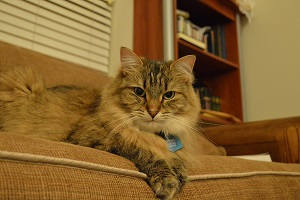
\includegraphics[width=0.365\textwidth]{./images/muffins_300x200.jpg}} & \fbox{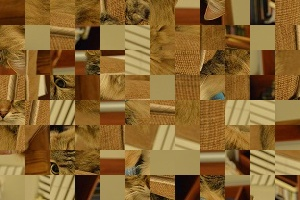
\includegraphics[width=0.365\textwidth]{./images/muffins_scrambled.jpg}}
	\\ ~\\
	(a) Ground-Truth Image & (b) Randomized Jig Swap Puzzle
	\\ ~\\
  \end{tabular}
\caption{Jig Swap Puzzle Example}
\label{fig:jigSwapExample}
\end{figure}

This thesis proposes a fully-automated solver for the simultaneous assembly of multiple jigsaw puzzles, with an overview of the architecture provided in Chapter~\ref{chap:mixedBagSolver}.  Chapter~\ref{chap:quantifyingSolverQuantify} presents a set of new metrics specifically tailored for quantifying the quality of outputs of multiple puzzle solvers; the chapter also outlines a set of standards for visualizing the characteristics of solver outputs.  Lastly, Chapter~\ref{chap:experimentalResults} compares the performance of this new solver with the current state of the art.